\section{Differential Equations}
Differential equations are equations, or sometimes systems of equations where we are given how a function relates to its derivatives and would like to find satisfying functions or families of functions.
Differential equations land themselves well to modeling real-world phenomena and are still an area of active mathematical study.
We'll see some very basic differential equations and how what we've learned about integrals can be used to solve them.

\subsection{Separable Differential Equations}
If we can break up a first-order (just involving a first derivative) ordinary differential equation into the following form,
\begin{equation*}
	\dd{y}{x} = f(x)g(y)
\end{equation*}
then we say the differential equation is separable and may be able to be solved using a technique called separation of variables.
The steps to solve a separable differential equation are:
\begin{enumerate}
	\item Write the equation in differential form (i.e using $\dd{y}{x}$)
	\item Separate the variables ($\frac{\d{y}}{g(y)}=f(x)\d{x}$)
	\item Integrate both sides
	\item Solve for $y$ in terms of $x$, if possible
	\item Find the general solution
	\item Find a particular solution, given any initial conditions
\end{enumerate}

\begin{example}
	Solve the following differential equation.
	\begin{equation*}
		\dd{y}{x} = (xy)^2, y(1)=1.
	\end{equation*}
\end{example}
\begin{answer}
	Separating and integrating,
	\begin{align*}
		\dd{y}{x} &= (xy)^2 = x^2y^2 \\
		\frac{\d{y}}{y^2} &= x^2\d{x} \\
		\frac{1}{y} &= \frac{x^3}{3} + C. \\
	\end{align*}
	
	Solving for $C$,
	\begin{align*}
		\frac{-1}{1} &= \frac{1^3}{3} + C \\
		C &= \frac{-4}{3}.
	\end{align*}
	
	Solving for $y$,
	\begin{align*}
		\frac{-1}{y} &= \frac{x^3}{3} - \frac{4}{3} \\
		y &= \frac{-3}{x^3 - 4}.
	\end{align*}
\end{answer}

\subsubsection{Exponential Growth \& Decay}
We can use differential equations to model growth and decay.

\begin{example}
	Imagine we have some money in a bank account earning interest.
	The more money in the bank, the more the more the account will receive in interest.
	So, the rate of growth of the account value is proportional to the current account value.
	In the language of differential equations,
	\begin{equation*}
		\dd{y}{t} = ky
	\end{equation*}
	where $k$ is some constant of proportionality.
\end{example}
\begin{answer}
	This equation is separable, so we'll try to solve it using separation of variables.
	\begin{align*}
		\frac{\d{y}}{t} &= k\d{x} \\
		\ln{\abs{y}} &= kt + C \\
		\abs{y} &= Ce^{kt} \\
		y &= Ce^{kt} \\
		y(0) &= Ce^{k\cdot 0} = C \\
		y &= y_0e^{kt}.
	\end{align*}
\end{answer}

This is exactly the equation for continually compounding interest: $y_0$ is the principle and $k$ is an interest rate.


Note that $k$ could theoretically be negative, meaning the amount would decrease proportionally to the remaining amount.
\begin{example}
	The half-life of Pu-239 is 24360 years.
	Suppose that 10g of Pu-239 were released in a nuclear accident, how long would it take to decay to 1g?
\end{example}
\begin{answer}
	Our ``principle'' is 10g.
	We know that half-life follows the exponential decay differential equation, so it's modeled by $y = 10e^{kt}$.
	We also know that $y(24360)=5$, which should give us enough information to solve for $k$.
	\begin{align*}
		5 &= 10e^{k\cdot 24360} \\
		\frac{1}{2} &= e^{k\cdot 24360} \text{ (see the ``half`` in half-life?)} \\
''		\ln{\frac{1}{2}} &= 24360k \\
		-\ln{2} &= 24360k \\
		k &= \frac{-\ln{2}}{24360}.
	\end{align*}
	
	We now can plug $k$ back into our equation to get the full model.
	\begin{align*}
		y &= 10e^{\frac{-\ln{2}}{24360}t} \\
		&= 10\left(e^{\ln{2}}\right)^{\frac{-t}{24360}} \\
		&= 10\cdot2^{-\frac{-t}{24360}}.
	\end{align*}
	
	We can now plug in 1 for $y$ and solve for $t$
	\begin{align*}
		1 &= 10\cdot2^{-\frac{t}{24360}} \\
		\frac{1}{10} &= 2^{-\frac{t}{24360}} \\
		\log_{2}{\frac{1}{10}} &= -\frac{t}{24360} \\
		\log_{2}{10} &= \frac{t}{24360} \\
		t &= 24360\log_{2}{10} \approx 80922\text{yr}.
	\end{align*}
	
	If you're familiar with half-life equations, this is exactly $t=t_{1/2}\log_{2}{\frac{N_0}{N_f}}$.
\end{answer}

\subsubsection{Logistic Growth \& Decay}
Although our differential equations assuming that growth is proportional to amount work well for things like bank accounts, bacteria or radioactive particles that can grow and decay without limits, that model is a little too simplistic to model populations that are limited by resources.

\begin{example}
	Imagine that we have a population of animals in a forest.
	If the forest has lots of resources to support to animal population, then they can grow basically like normal.
	However, as the population grows, resources become more scarce, so population growth would slow down, or some of the population would starve.
	We can model this with the following differential equation.
	\begin{equation*}
		\dd{P}{t} = kP(M-P)
	\end{equation*}
	where $k$ is some constant of proportionality and $M$ is some maximum population before growth starts to decline.
\end{example}
\begin{answer}
	This differential equation is also separable, so let's try to solve it.
	\begin{align*}
		\dd{P}{t} &= kP(M-P) \\
		\frac{\d{P}}{P(M-P)} &= k\d{t} \\
		\d{P}\left(\frac{1/M}{P}+\frac{1/M}{M-P}\right) &= k\d{t} \text{ (using partial fractions)} \\
		\frac{1}{M}\left(\ln{\abs{P}} - \ln{\abs{M-P}}\right) &= kt + C \\
		\ln{\abs{\frac{P}{M-P}}} &= Mkt + C \\
		\frac{P}{M-P} &= Ce^{Mkt} \text{ (b/c $P \geq 0$)} \\
		P &= CMe^{Mkt} - CPe^{Mkt} \\
		P\left(1+Ce^{Mkt}\right) &= CMe^{Mkt} \\
		P &= \frac{CMe^{Mkt}}{1+Ce^{Mkt}} \\
		&= \frac{M}{1+Ce^{-Mkt}}.
	\end{align*}
\end{answer}

\begin{figure}[H]
	\label{logistic}
	\centering
	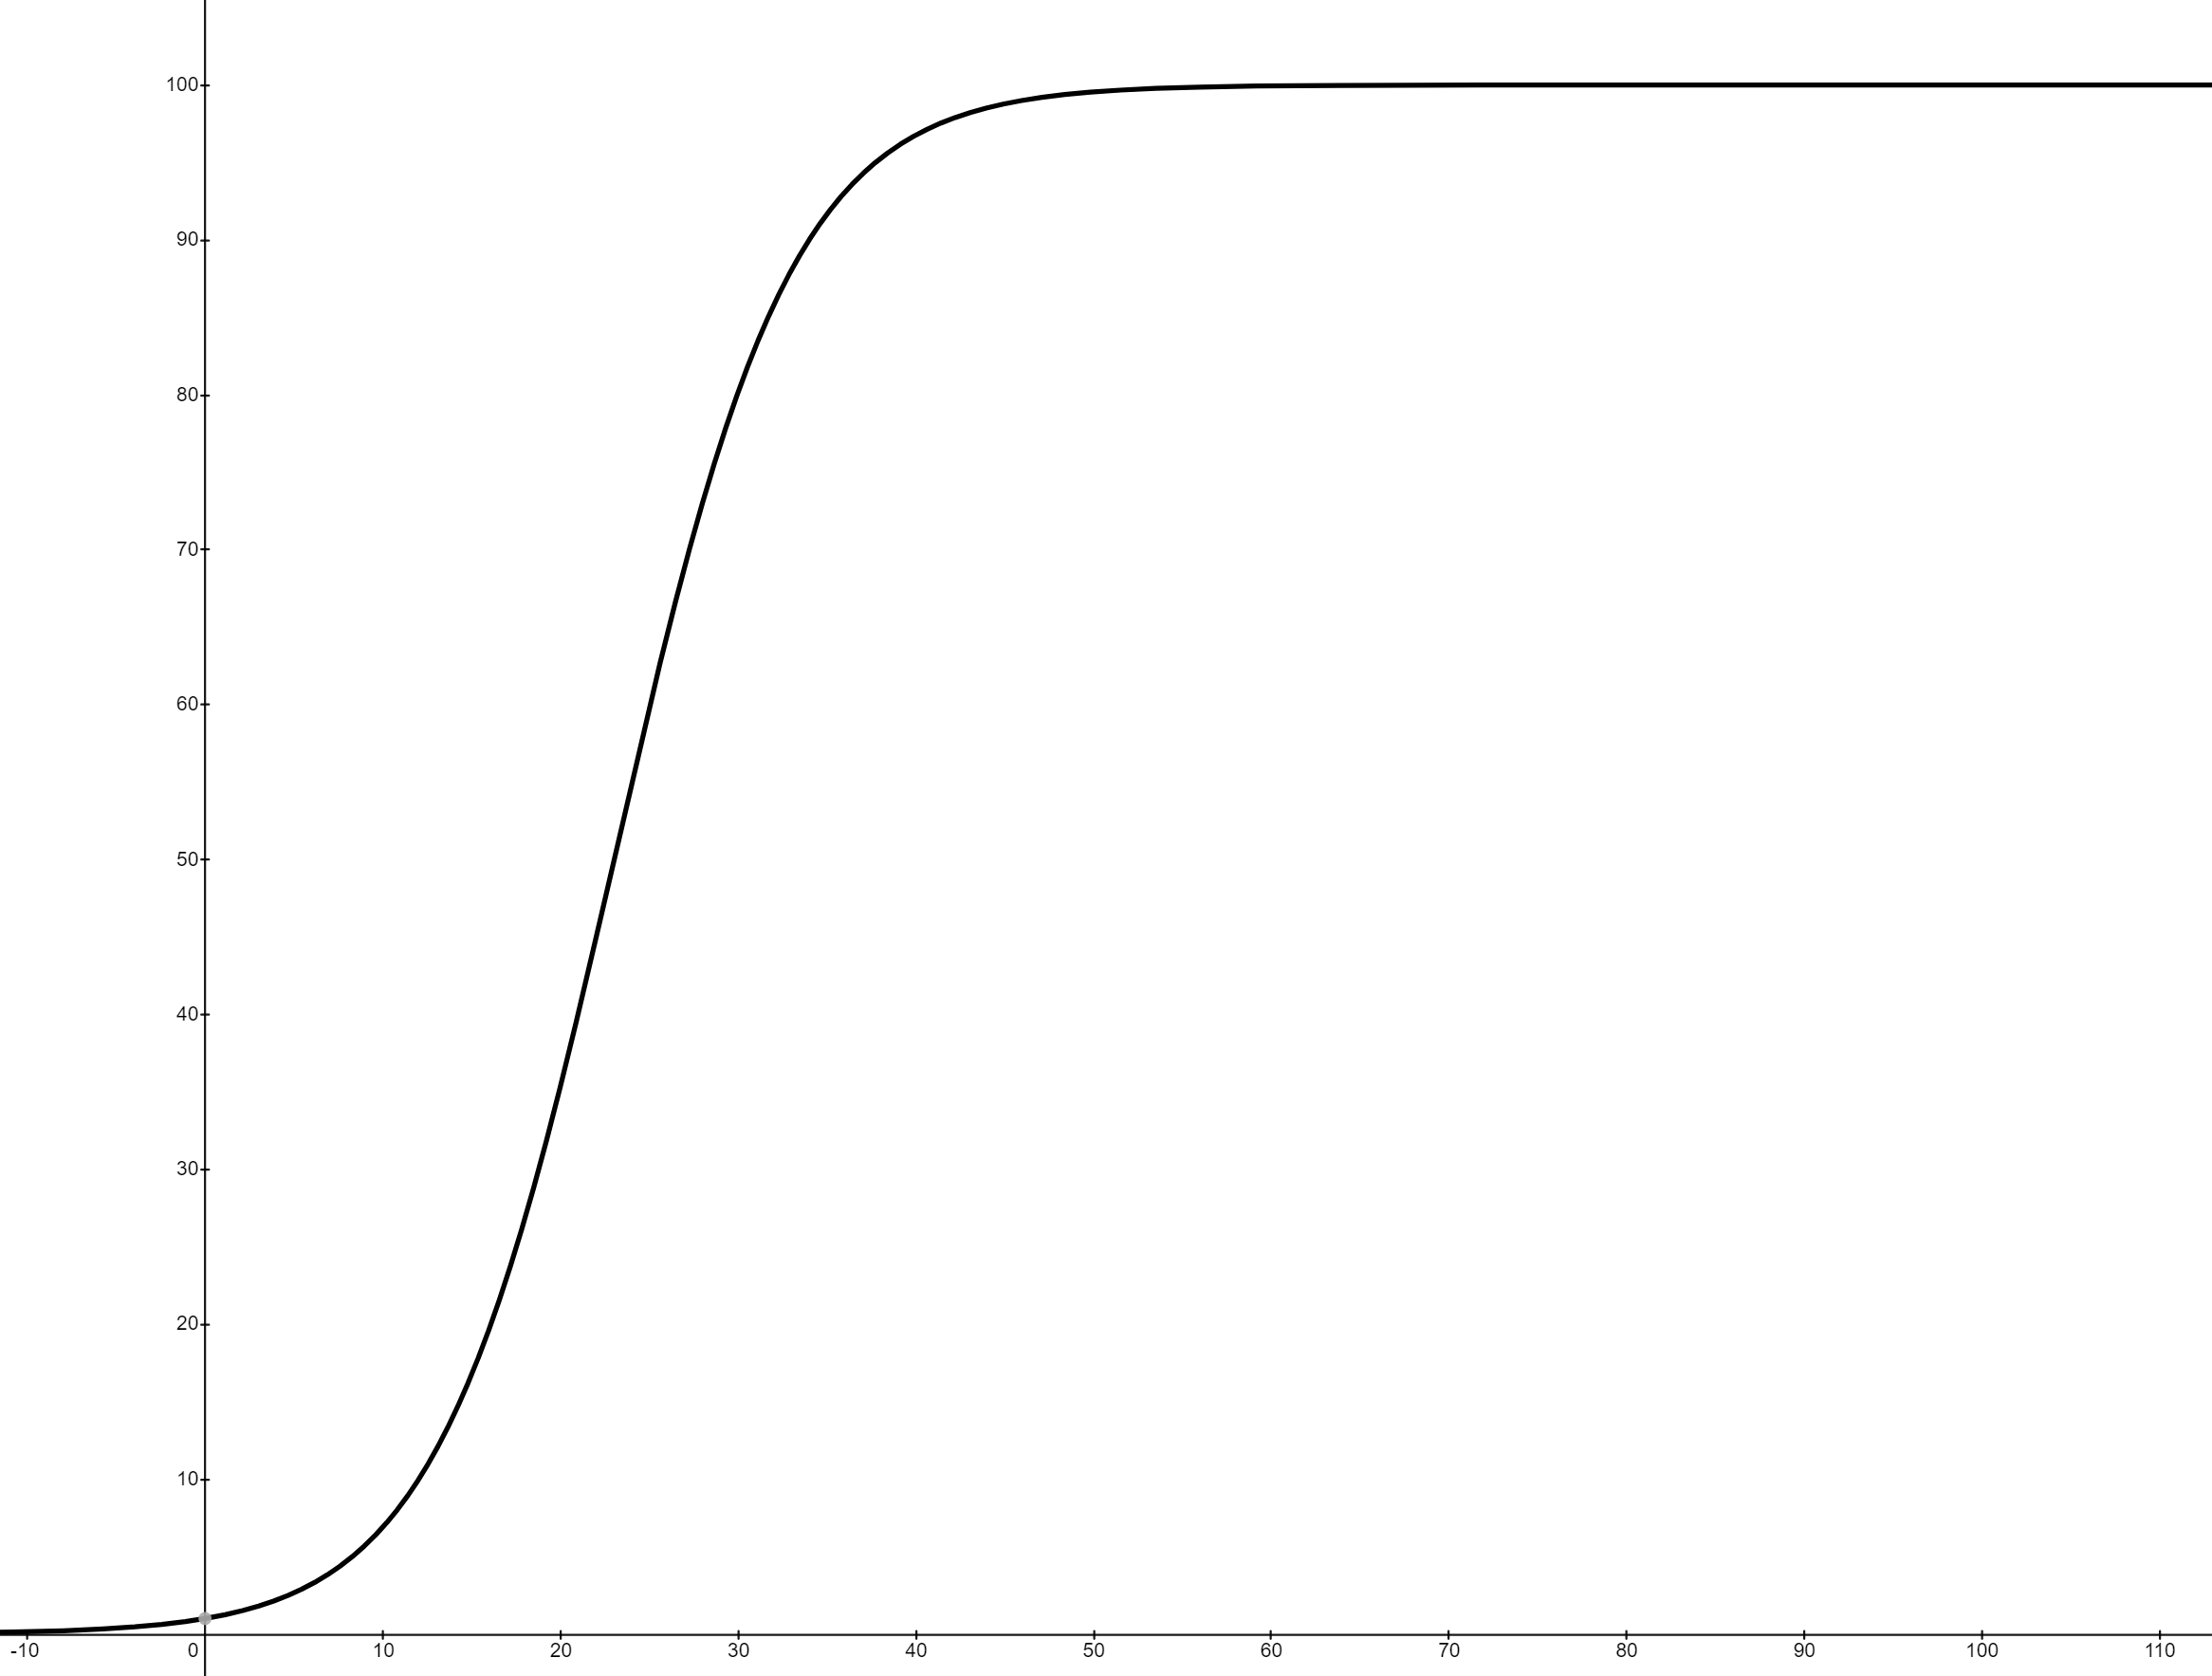
\includegraphics[width=0.5\textwidth]{./applications_integrals/logistic_growth.png}
	\caption{\hyperref{}{}{}{Logistic Growth}}
\end{figure}

Looking at a graph of this function, we can see that it starts growing like an exponential curve but begins to flatten, obtaining a maximum value of $M$, which is called the carrying capacity.
The population is growing the fastest when $P=M/2$, which you can verify by finding the global maxima of $\dd{P}{t}$ using a first derivative test.

\subsection{Slope Fields \& Euler's Method}
Unfortunately, not all differential equations are as easy to solve as separable differential equations.
In fact, some are impossible to get nice, closed-form solutions.
\subsubsection{Slope Fields}
We may still be able to visualize what the graph of a solution might look like by drawing lines that have the same slope as a solution.
Any solution that passes through the points where we draw the sloped lines must be tangent to these lines, meaning a solution will follow the ``flow`` of these lines.
''
\begin{figure}[H]
	\label{slope_field}
	\centering
	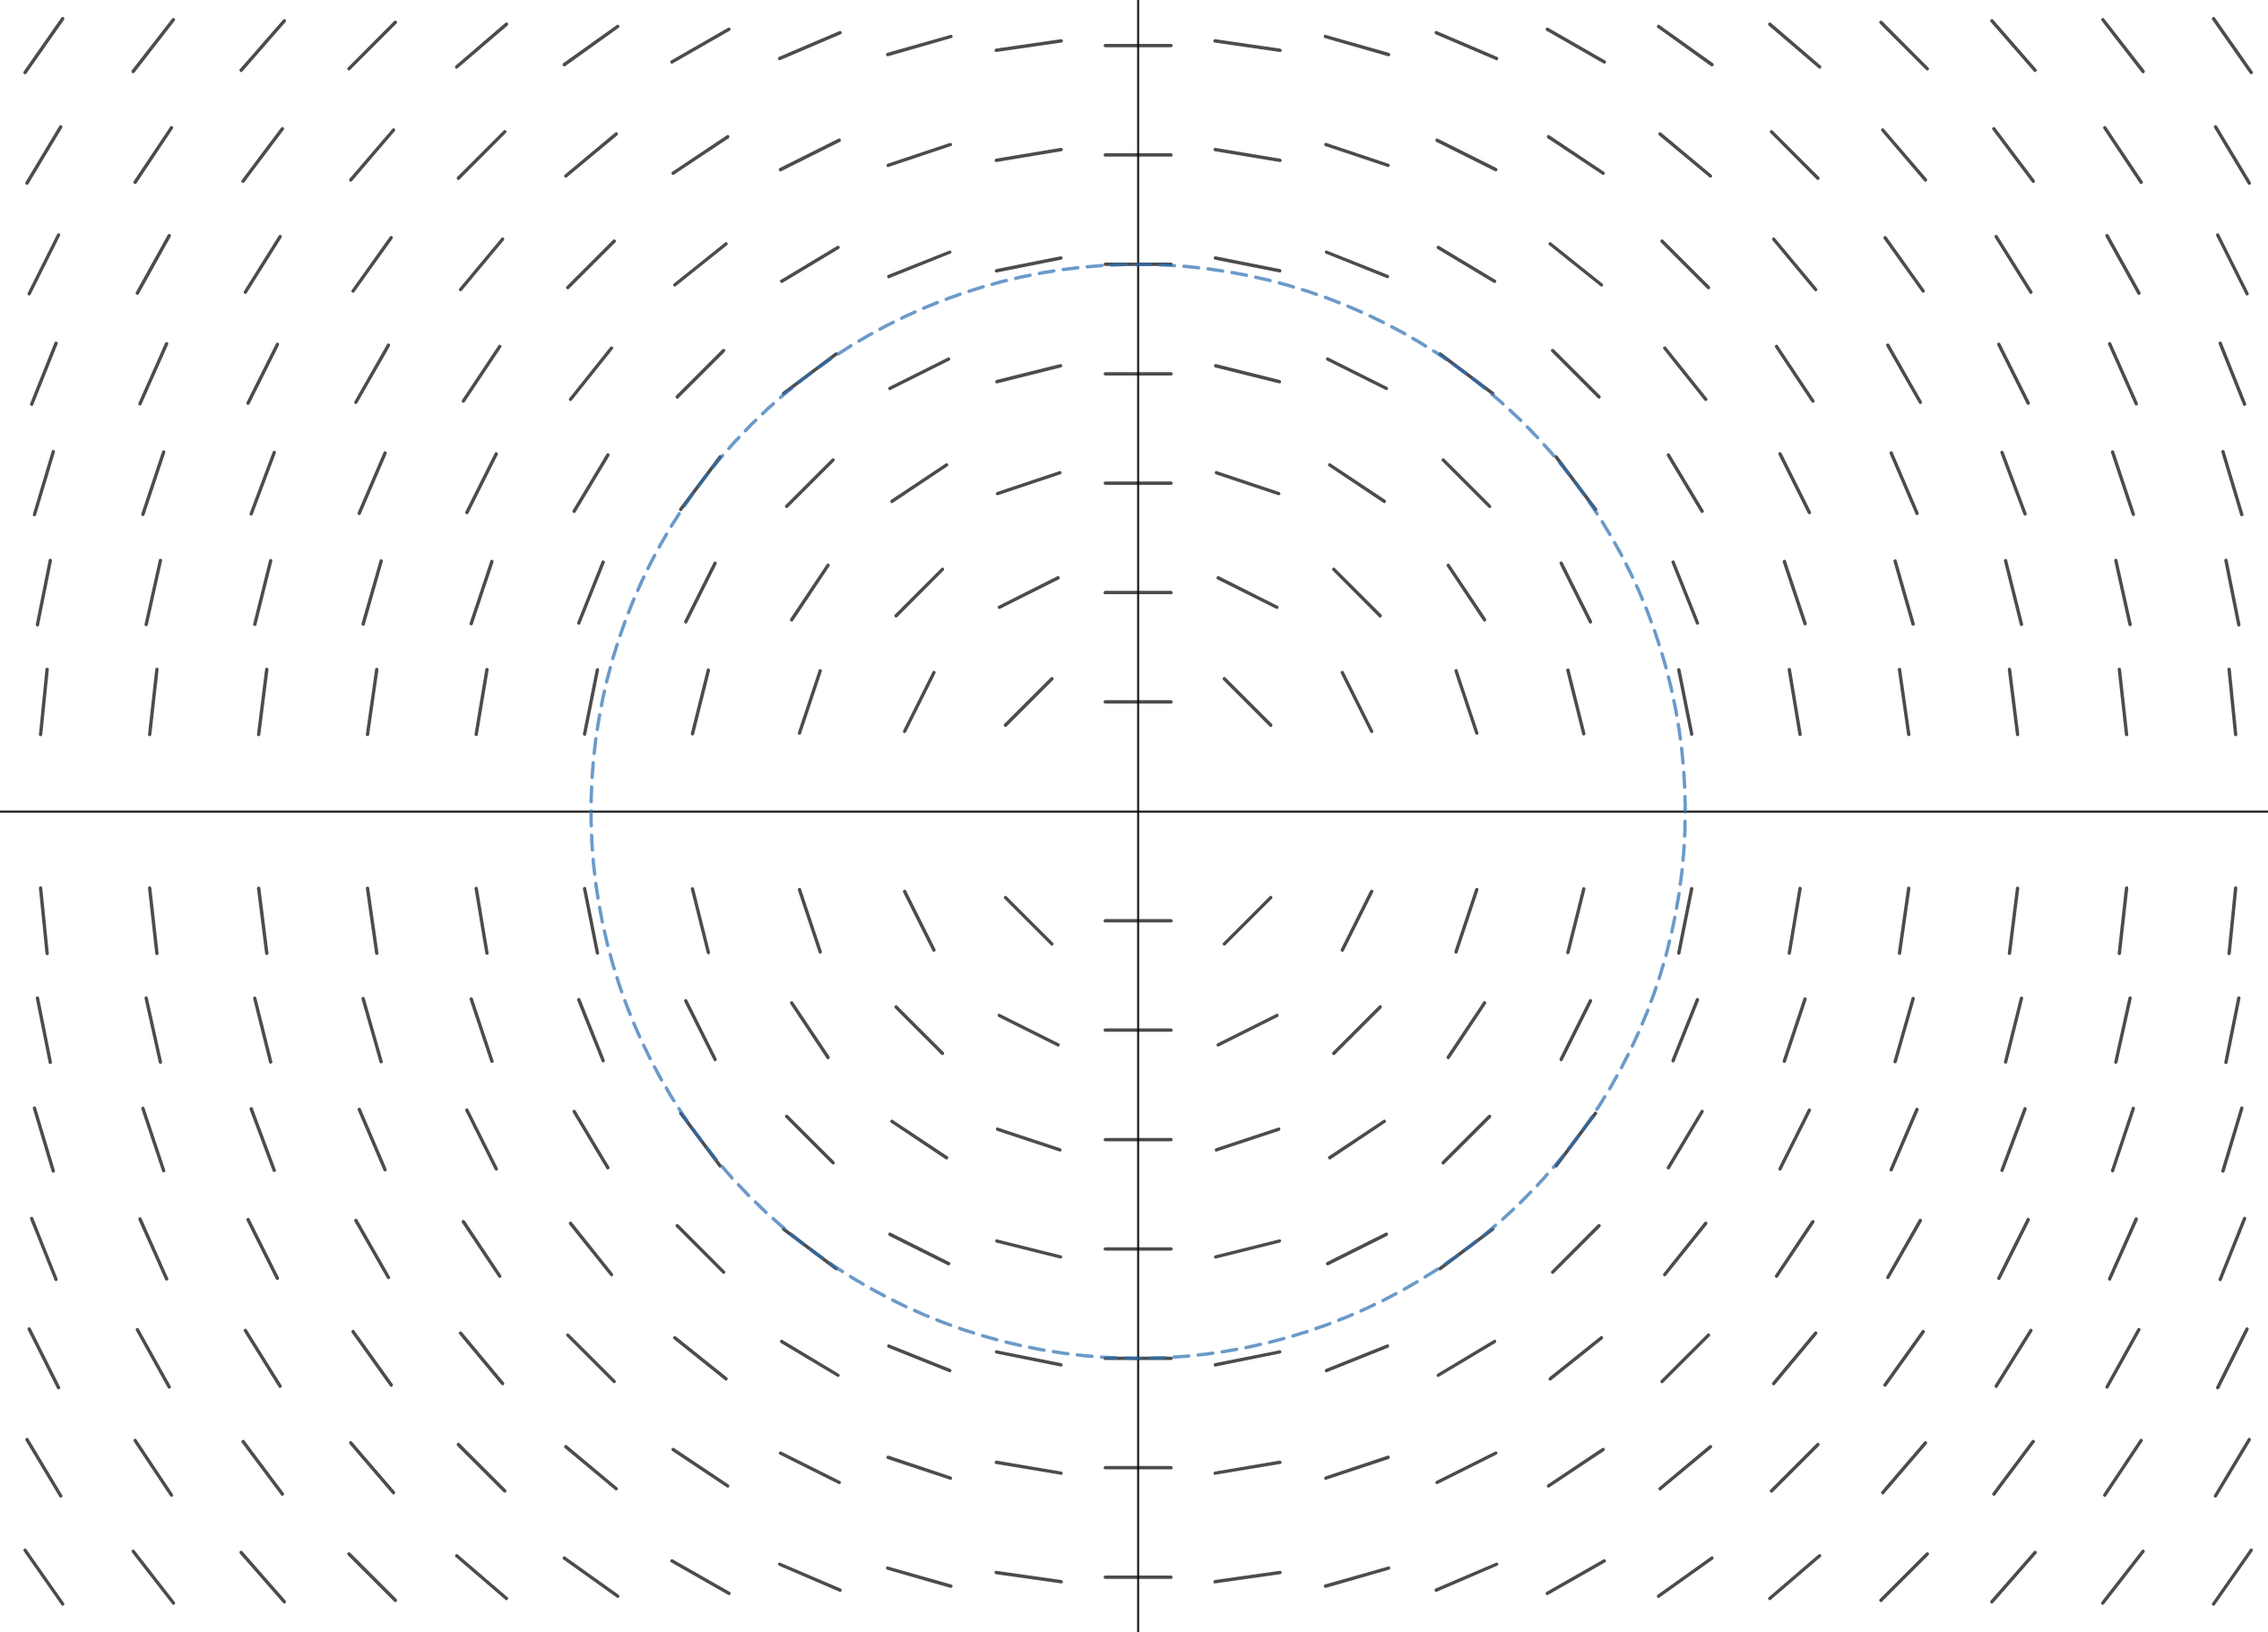
\includegraphics[width=0.75\textwidth]{./applications_integrals/slope_field.png}
	\caption{\hyperref{}{}{}{Slope field of $\dd{y}{x}=-x/y$ with a possible solution}}
\end{figure}

\subsubsection{Euler's Method}
If your differential equation also has an initial condition, you can start at the initial point and follow the slope field to find an approximate solution.
This is what Euler's Method tries to accomplish.
It can approximate the value of a solution at some $x$ value by starting at some point, usually given by the initial condition, and iteratively taking small steps of size $\Delta x$ in the direction determined by the slope field.
\begin{align*}
	x_{n+1} &= x_n + \Delta x \\
	y_{n+1} &= y_n + \Delta x\dd{y}{x}_{(x_n,y_n)}.
\end{align*}

The smaller the steps, the more accurate the approximation.
\begin{figure}[H]
	\label{eulers_method}
	\centering
	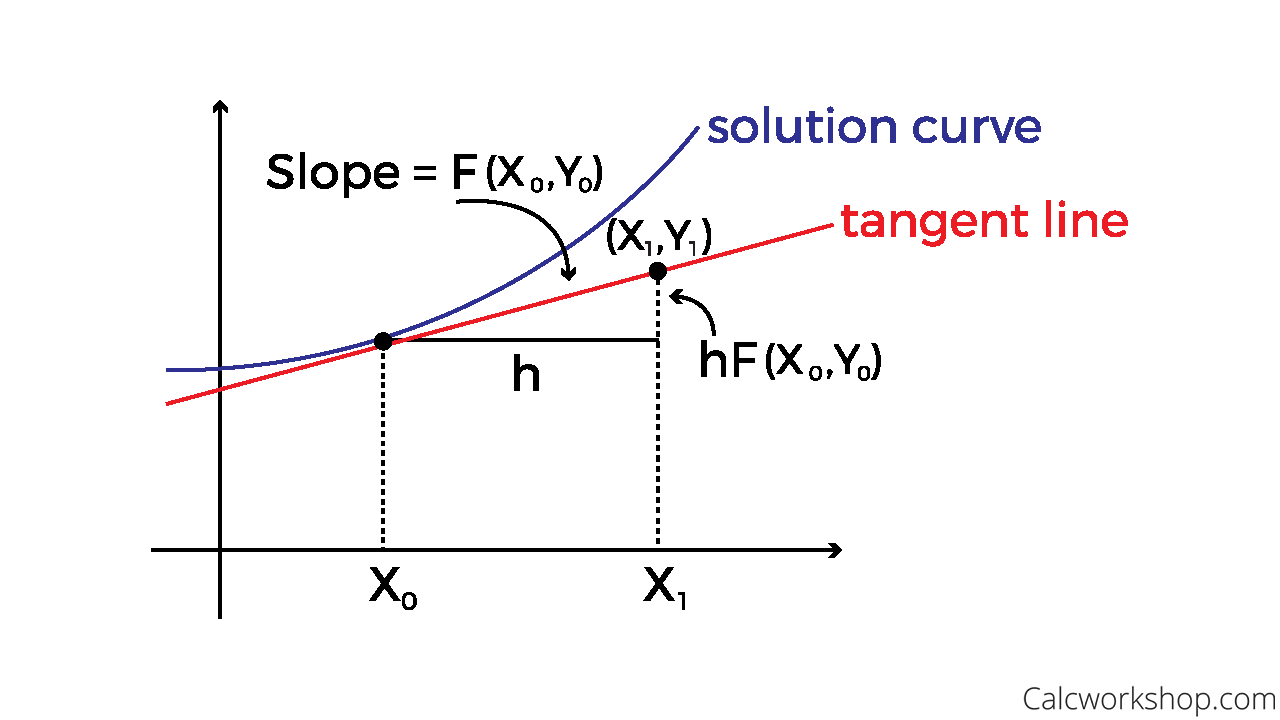
\includegraphics[width=0.55\textwidth]{./applications_integrals/Eulers-Approximation.png}
	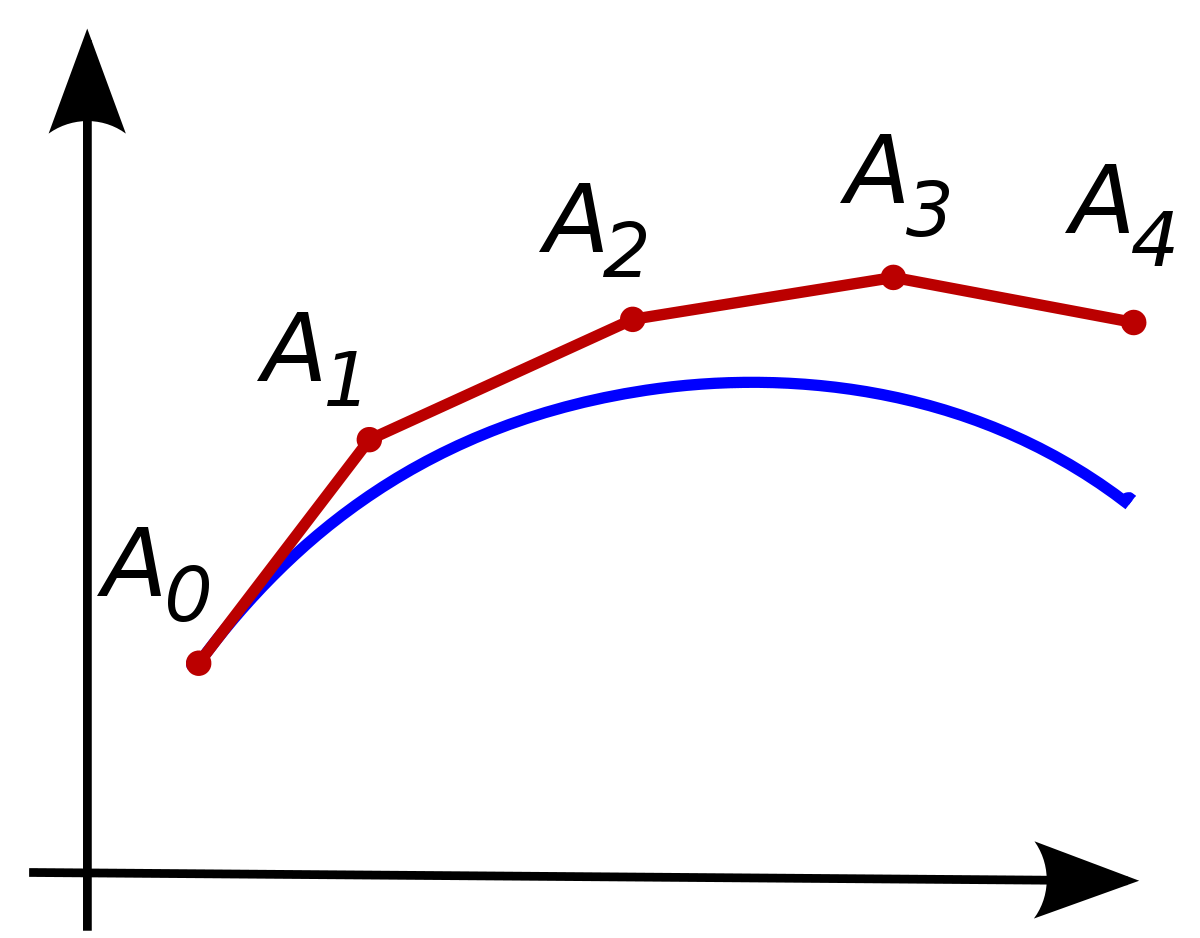
\includegraphics[width=0.35\textwidth]{./applications_integrals/Eulers-Approximation2.png}
	\caption{\hyperref{https://calcworkshop.com/first-order-differential-equations/eulers-method-table/}{}{}{Calc Workshop - Euler's Method};\hspace{5pt}\hyperref{https://en.wikipedia.org/wiki/Euler\_method}{}{}{Wikipedia - Euler Method}}
\end{figure}

\begin{example}
	Given that $\dd{y}{x}=3-x$ and $y(4)=2$, approximate the value of $y(5)$ using Euler's method with increments of $\Delta x = 0.25$.
\end{example}
\begin{answer}
	\begin{table}[H]
		\begin{center}
			\begin{tabular}{|c|c|c|c|c|}
				\hline
				$(x,y)$ & $\dd{y}{x}$ & $\Delta x$ & $\Delta y = \Delta x\dd{y}{x}$ & $(x+\Delta x, y+\Delta y)$ \\
				\hline
				$(4,2)$ & $-1$ & $0.25$ & $-0.25$ & $(4.25,1.75)$ \\
				\hline
				$(4.25,1.75)$ & $-1.25$ & $0.25$ & $-0.3125$ & $(4.5,1.4375)$ \\
				\hline
				$(4.5,1.4375)$ & $-1.5$ & $0.25$ & $-0.375$ & $(4.75,1.0625)$ \\
				\hline
				$(4.75,1.0625)$ & $-1.75$ & $0.25$ & $-0.4375$ & $(5,0.625)$ \\
				\hline
			\end{tabular}
		\end{center}
	\end{table}
	
	So, Euler's Method yields an approximate\footnote{The actual value of the solution is $(5,0.5)$, so not too far off.} value of $(5,0.625)$.
\end{answer}